\documentclass[12pt]{article}

% Packages
\usepackage[margin=1in]{geometry}
\usepackage{graphicx}
\usepackage{booktabs}
\usepackage{amsmath}
\usepackage{natbib}
\usepackage{setspace}
\usepackage[hidelinks]{hyperref}
\usepackage{float}
\usepackage{caption}
\usepackage{subcaption}
\usepackage[table]{xcolor}
\usepackage{enumitem}
\usepackage{parskip}
\usepackage{multirow}

% Formatting
\singlespacing
\setlength{\parindent}{0pt}
\setlength{\parskip}{4pt}
\captionsetup{font=small, skip=4pt}

% Title
\title{\textbf{Descriptive Statistics Analysis of the Mnemonic Similarity Task (MST):\\Examining Pattern Separation Across Encoding Conditions}}
\author{\textbf{Team Data Navigators} \\
Sourav Nath (Roll: 2025201054) \\
Piyush Kumar Agarwal (Roll: 2025201082) \\
Rajarshi Chatterjee (Roll: 2025814004) \\\\
BRSM 2026}
\date{\today}

\begin{document}

\maketitle

% ============================================================
% INTRODUCTION
% ============================================================
\section{Introduction}

The ability to distinguish between highly similar yet distinct experiences is fundamental to human memory, a process known as \textit{pattern separation} \citep{yassa2011pattern}. Attributed primarily to the hippocampal dentate gyrus, pattern separation transforms overlapping memory representations into distinct neural codes, preventing memory interference \citep{bakker2008pattern}.

The \textbf{Mnemonic Similarity Task (MST)} \citep{stark2013mnemonic} is a widely used paradigm for assessing pattern separation. It consists of an \textit{encoding phase} (viewing object/scene images) and a \textit{recognition test} with three stimulus types: 
\begin{itemize}[nosep, leftmargin=1.5em]
\item \textbf{Targets} (exact repetitions; expected response: ``Old'') 
\item \textbf{Lures} (similar but not identical items, varied across similarity bins 1--5; expected response: ``Similar'')
\item \textbf{Foils} (novel items; expected response: ``New'').
\end{itemize}
Our dataset comprises 160 participants across three between-subjects encoding conditions: 
\begin{itemize}[nosep, leftmargin=1.5em]
\item \textit{Item Only} ($N = 56$; indoor/outdoor item judgments)
\item \textit{Task Only} ($N = 53$; task-based encoding)
\item \textit{Both} ($N = 51$; combined item and task encoding). 
\end{itemize}
Each participant encoded 192 stimuli (objects and scenes) and completed $\sim$150 test trials. This report presents a thorough descriptive statistical analysis of MST performance, examining key metrics, response distributions, reaction times, and similarity-dependent lure discrimination.

% ============================================================
% METHODS
% ============================================================
\section{Methods}

\subsection{Dataset Description}

The dataset comprises behavioral responses from $N = 160$ participants assigned to three between-subject encoding conditions. Data for each participant is stored in individual CSV files. Each row in the dataset represents a single test-phase trial, recording the stimulus presented, its actual category (Target, Lure, or Foil), the participant's keypress response (Old, Similar, New), and the corresponding reaction time in seconds. For this preliminary descriptive analysis, the dataset was analyzed in its raw, complete form; no participant-level outlier exclusions or data imputations for missing trials were applied, ensuring the descriptive statistics reflect the unfiltered behavioral responses.

\subsection{Experiment Design}

This study employed a \textbf{between-subjects design} with three encoding conditions. The variables are defined as follows:

\textbf{Independent Variable:} Encoding Condition (Item Only / Task Only / Both).

\textbf{Dependent Variables:}
\begin{itemize}[nosep, leftmargin=1.5em]
    \item Lure Discrimination Index (LDI) --- primary measure of pattern separation
    \item Recognition Memory (REC) --- measure of old/new discrimination
    \item Hit Rate --- proportion of targets correctly identified as ``Old''
    \item Reaction Time (RT) --- response latency across stimulus types
\end{itemize}

Participants ($N = 160$) were assigned to one of three conditions: \textit{Item Only} ($N = 56$; indoor/outdoor item judgments during encoding), \textit{Task Only} ($N = 53$; task-based procedural encoding), or \textit{Both} ($N = 51$; combined item and task encoding). Each participant encoded 192 stimuli (objects and scenes) and completed approximately 150 test trials with three response options: ``Old,'' ``Similar,'' or ``New.''

\subsection{Hypotheses}

Based on the pattern separation framework and prior MST literature, we tested the following hypotheses:

\textbf{Hypothesis 1 (Pattern Separation):}
\begin{quote}
$H_0$: LDI $= 0$ (no pattern separation; lure discrimination equals foil response bias).\\
$H_1$: LDI $> 0$ (significant pattern separation; participants can distinguish lures from foils).\\
\textit{Test:} One-sample $t$-test (one-tailed) per condition.
\end{quote}

\newpage
\textbf{Hypothesis 2 (Recognition Memory):}
\begin{quote}
$H_0$: REC $= 0$ (no recognition memory; hit rate equals false alarm rate).\\
$H_1$: REC $> 0$ (significant recognition memory; participants correctly identify targets).\\
\textit{Test:} One-sample $t$-test (one-tailed) per condition.
\end{quote}

\textbf{Hypothesis 3 (Similarity Effect on Lure Discrimination):}
\begin{quote}
$H_0$: Lure discrimination does not vary across similarity bins (1--5).\\
$H_1$: Higher-similarity lures (Bin~1) are harder to discriminate than lower-similarity lures (Bin~5).\\
\textit{Test:} Descriptive analysis of response proportions across similarity bins.
\end{quote}

\subsection{Data Processing}

All analyses were conducted in R (v4.5.2) using R Markdown. Test-phase CSV files from all conditions were loaded programmatically. Stimuli were classified as \textit{Target} (``a''-suffix images from encoding), \textit{Lure} (``b''-suffix similar versions), or \textit{Foil} (novel images from Foils folder). Responses were coded as ``Old'' (o), ``Similar'' (s), or ``New'' (n). Lure items were matched to similarity bins (1--5) using provided mapping files.

\subsection{Performance Metrics}

Per-participant metrics included:  
\begin{itemize}[nosep, leftmargin=1.5em]
\item \textbf{Hit Rate} $= P(\text{``Old''} \mid \text{Target})$
\item \textbf{False Alarm Rate} $= P(\text{``Old''} \mid \text{Foil})$
\item \textbf{Correct Rejection Rate} $= P(\text{``New''} \mid \text{Foil})$ 
\item \textbf{Lure Discrimination Index}:
\begin{equation}
    \text{LDI} = P(\text{``Similar''} \mid \text{Lure}) - P(\text{``Similar''} \mid \text{Foil})
\end{equation}
which quantifies pattern separation corrected for response bias \citep{stark2013mnemonic}
\item \textbf{Recognition Memory}:
\begin{equation}
    \text{REC} = P(\text{``Old''} \mid \text{Target}) - P(\text{``Old''} \mid \text{Foil})
\end{equation}
\end{itemize}
\subsection{Statistical Approach}

Descriptive statistics (mean, SD, median) were computed for all metrics. One-sample $t$-tests evaluated whether LDI and REC exceeded zero, with Cohen's $d$ as effect size. Reaction times were analyzed after excluding values above the 99th percentile.

% ============================================================
% RESULTS
% ============================================================
\section{Results}

\subsection{Overall Performance}

Table~\ref{tab:summary} summarizes key metrics. All conditions showed robust recognition (REC $> .59$) and reliable lure discrimination (LDI $> .26$). Hit rates ranged from .627 to .669; false alarm rates were very low (.031--.047); correct rejection rates were high (.755--.775).

\begin{table}[H]
\centering
\caption{Summary Statistics by Condition (Mean $\pm$ SD)}
\label{tab:summary}
\footnotesize
\begin{tabular}{lccccc}
\toprule
\textbf{Condition} & \textbf{Hit Rate} & \textbf{FA Rate} & \textbf{LDI} & \textbf{REC} & \textbf{CR Rate} \\
\midrule
Item Only ($N\!=\!56$) & $.669 \pm .145$ & $.035 \pm .059$ & $.319 \pm .169$ & $.634 \pm .153$ & $.775 \pm .128$ \\
Task Only ($N\!=\!53$) & $.627 \pm .168$ & $.031 \pm .050$ & $.381 \pm .188$ & $.596 \pm .174$ & $.775 \pm .136$ \\
Both ($N\!=\!51$)      & $.642 \pm .133$ & $.047 \pm .071$ & $.269 \pm .175$ & $.594 \pm .139$ & $.755 \pm .117$ \\
\bottomrule
\end{tabular}
\end{table}

\subsection{Hypothesis Testing}


\textbf{H1 (Pattern Separation --- LDI $> 0$):} One-sample $t$-tests confirmed that LDI was significantly above zero in all conditions, leading to \textbf{rejection of $H_0$}: 
\begin{itemize}[nosep, leftmargin=1.5em]
\item Item Only, $t(55) = 14.09$, $p < .001$, $d = 1.88$
\item Task Only, $t(52) = 14.74$, $p < .001$, $d = 2.02$
\item Both, $t(50) = 10.96$, $p < .001$, $d = 1.54$. 
\end{itemize}
All effect sizes exceeded $d = 1.5$, indicating very large effects.

\textbf{H2 (Recognition Memory --- REC $> 0$):} REC was significantly positive in all conditions (all $t > 24$, $p < .001$), leading to \textbf{rejection of $H_0$}. Participants reliably distinguished targets from foils across all encoding conditions.

\textbf{H3 (Similarity Effect):} As detailed in Section~\ref{sec:bins}, bin analysis revealed the expected graded pattern---more similar lures were harder to discriminate---\textbf{supporting $H_1$}.

\subsection{Response Proportions}

Table~\ref{tab:resp_props} and Figure~\ref{fig:response_props} show response distributions. Targets were predominantly endorsed as ``Old'' (.627--.669), foils as ``New'' (.754--.775), and lures elicited the most ``Similar'' responses in Task Only (.574) and the fewest in Both (.466). \textbf{This pattern indicates that while baseline recognition memory remains remarkably stable across conditions, the capacity to resolve mnemonic interference (identifying lures) is highly sensitive to the nature of initial encoding.}

\begin{table}[H]
\centering
\caption{Response Proportions by Stimulus Type and Condition}
\label{tab:resp_props}
\footnotesize
\begin{tabular}{llccc}
\toprule
\textbf{Condition} & \textbf{Stimulus} & \textbf{P(``Old'')} & \textbf{P(``Similar'')} & \textbf{P(``New'')} \\
\midrule
\multirow{3}{*}{Item Only} & Target & .669 & .233 & .098 \\
                           & Lure   & .290 & .509 & .201 \\
                           & Foil   & .035 & .190 & .775 \\
\midrule
\multirow{3}{*}{Task Only} & Target & .627 & .270 & .103 \\
                           & Lure   & .247 & .574 & .178 \\
                           & Foil   & .031 & .194 & .775 \\
\midrule
\multirow{3}{*}{Both}      & Target & .638 & .247 & .114 \\
                           & Lure   & .305 & .466 & .229 \\
                           & Foil   & .047 & .199 & .754 \\
\bottomrule
\end{tabular}
\end{table}

\begin{figure}[H]
    \centering
    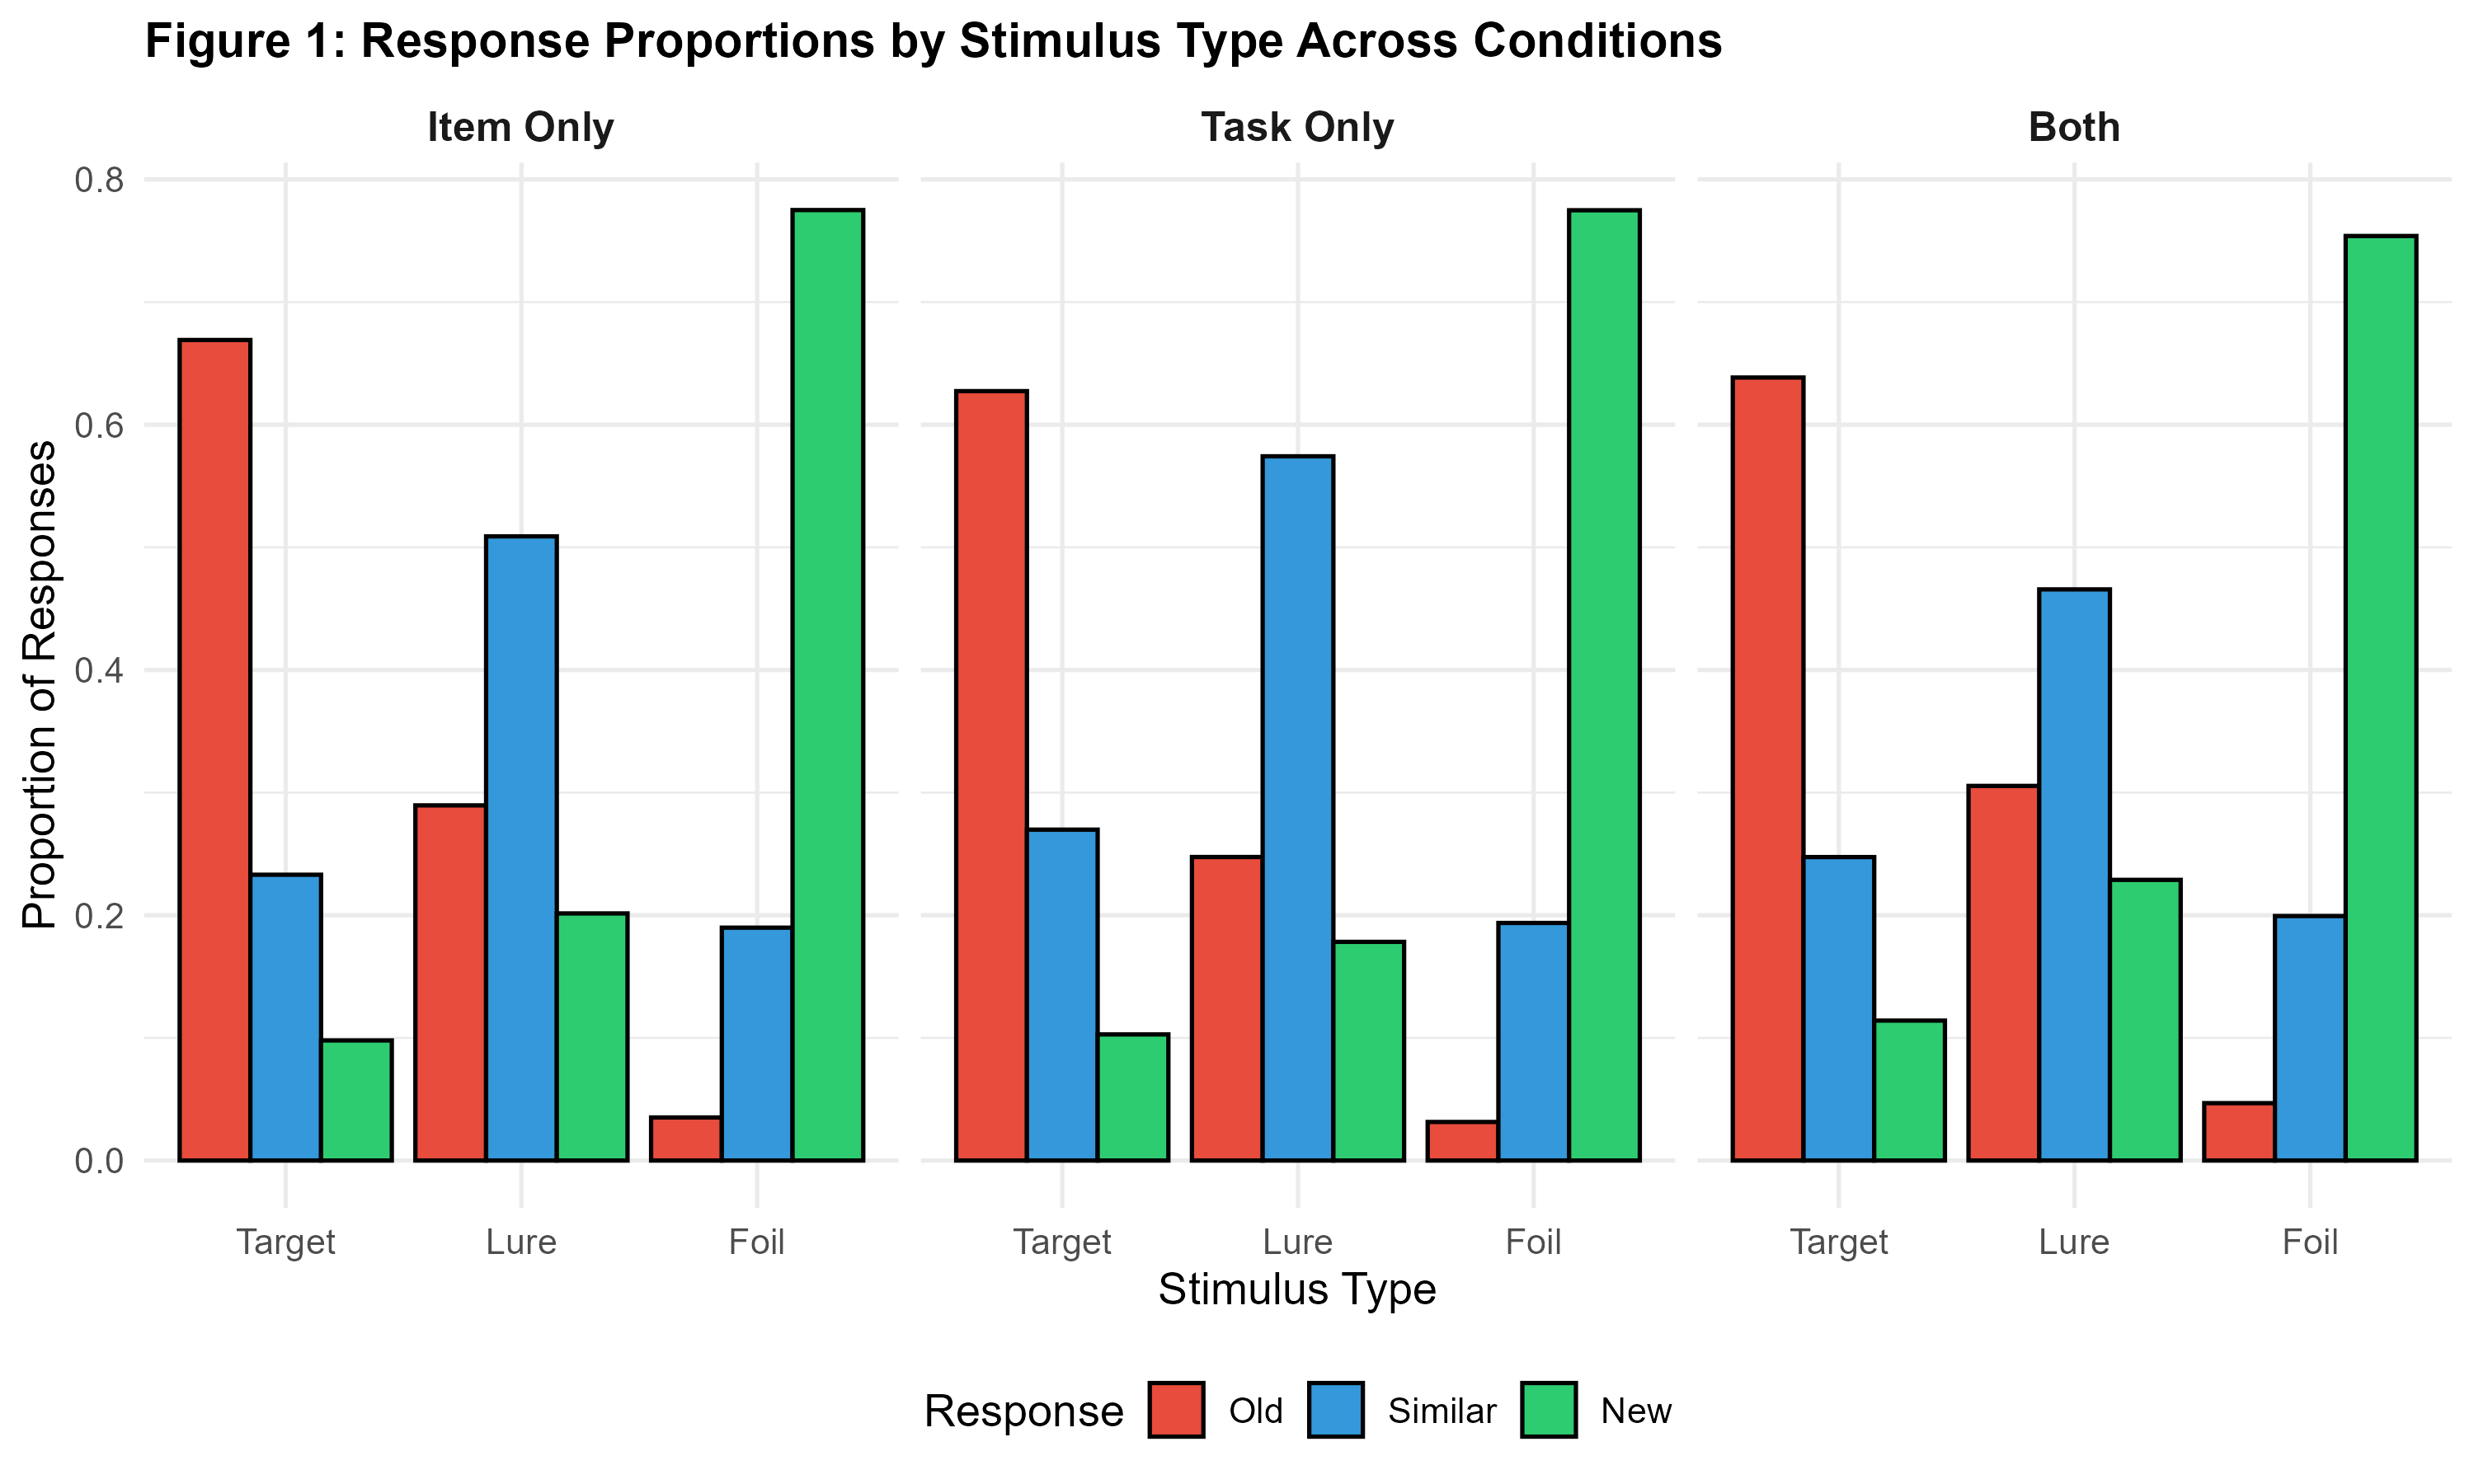
\includegraphics[width=0.85\textwidth]{figures/fig1_response_proportions.png}
    \caption{Response proportions by stimulus type across the three encoding conditions.}
    \label{fig:response_props}
\end{figure}

\subsection{LDI, REC, and Hit/FA Distributions}

Task Only exhibited the highest mean LDI (.381), followed by Item Only (.319) and Both (.269). REC scores were comparable across conditions (.594--.634). Figure~\ref{fig:metrics} displays the distributions of these key metrics. \textbf{Notably, the spread and interquartile range for LDI is visually wider than that of REC across all conditions. This suggests that while basic recognition is a relatively uniform capability among participants, pattern separation exhibits substantial individual differences and variance.}

\begin{figure}[H]
    \centering
    \begin{subfigure}[t]{0.48\textwidth}
        
\includegraphics[width=\textwidth]{figures/fig2_ldi_rec_boxplot.png}
        \caption{LDI and REC by condition}
    \end{subfigure}
    \hfill
    \begin{subfigure}[t]{0.48\textwidth}
        
\includegraphics[width=\textwidth]{figures/fig3_hit_fa_boxplot.png}
        \caption{Hit Rate and FA Rate by condition}
    \end{subfigure}
    \caption{Distribution of key performance metrics with individual participant data points overlaid.}
    \label{fig:metrics}
\end{figure}

\subsection{LDI Distribution and $t$-Distribution Fit}

LDI distributions were approximately normal in all conditions. Figure~\ref{fig:distributions} compares empirical distributions against fitted normal and $t$-distributions ($df = n-1$). Both provided excellent approximations, with the $t$-distribution offering slightly heavier tails to account for individual variation. \textbf{The confirmation of this approximately normal distribution is a crucial methodological step, as it formally justifies the use of parametric statistics (such as our one-sample $t$-tests) for evaluating pattern separation performance in this sample.}

\begin{figure}[H]
    \centering
    \begin{subfigure}[t]{0.48\textwidth}
        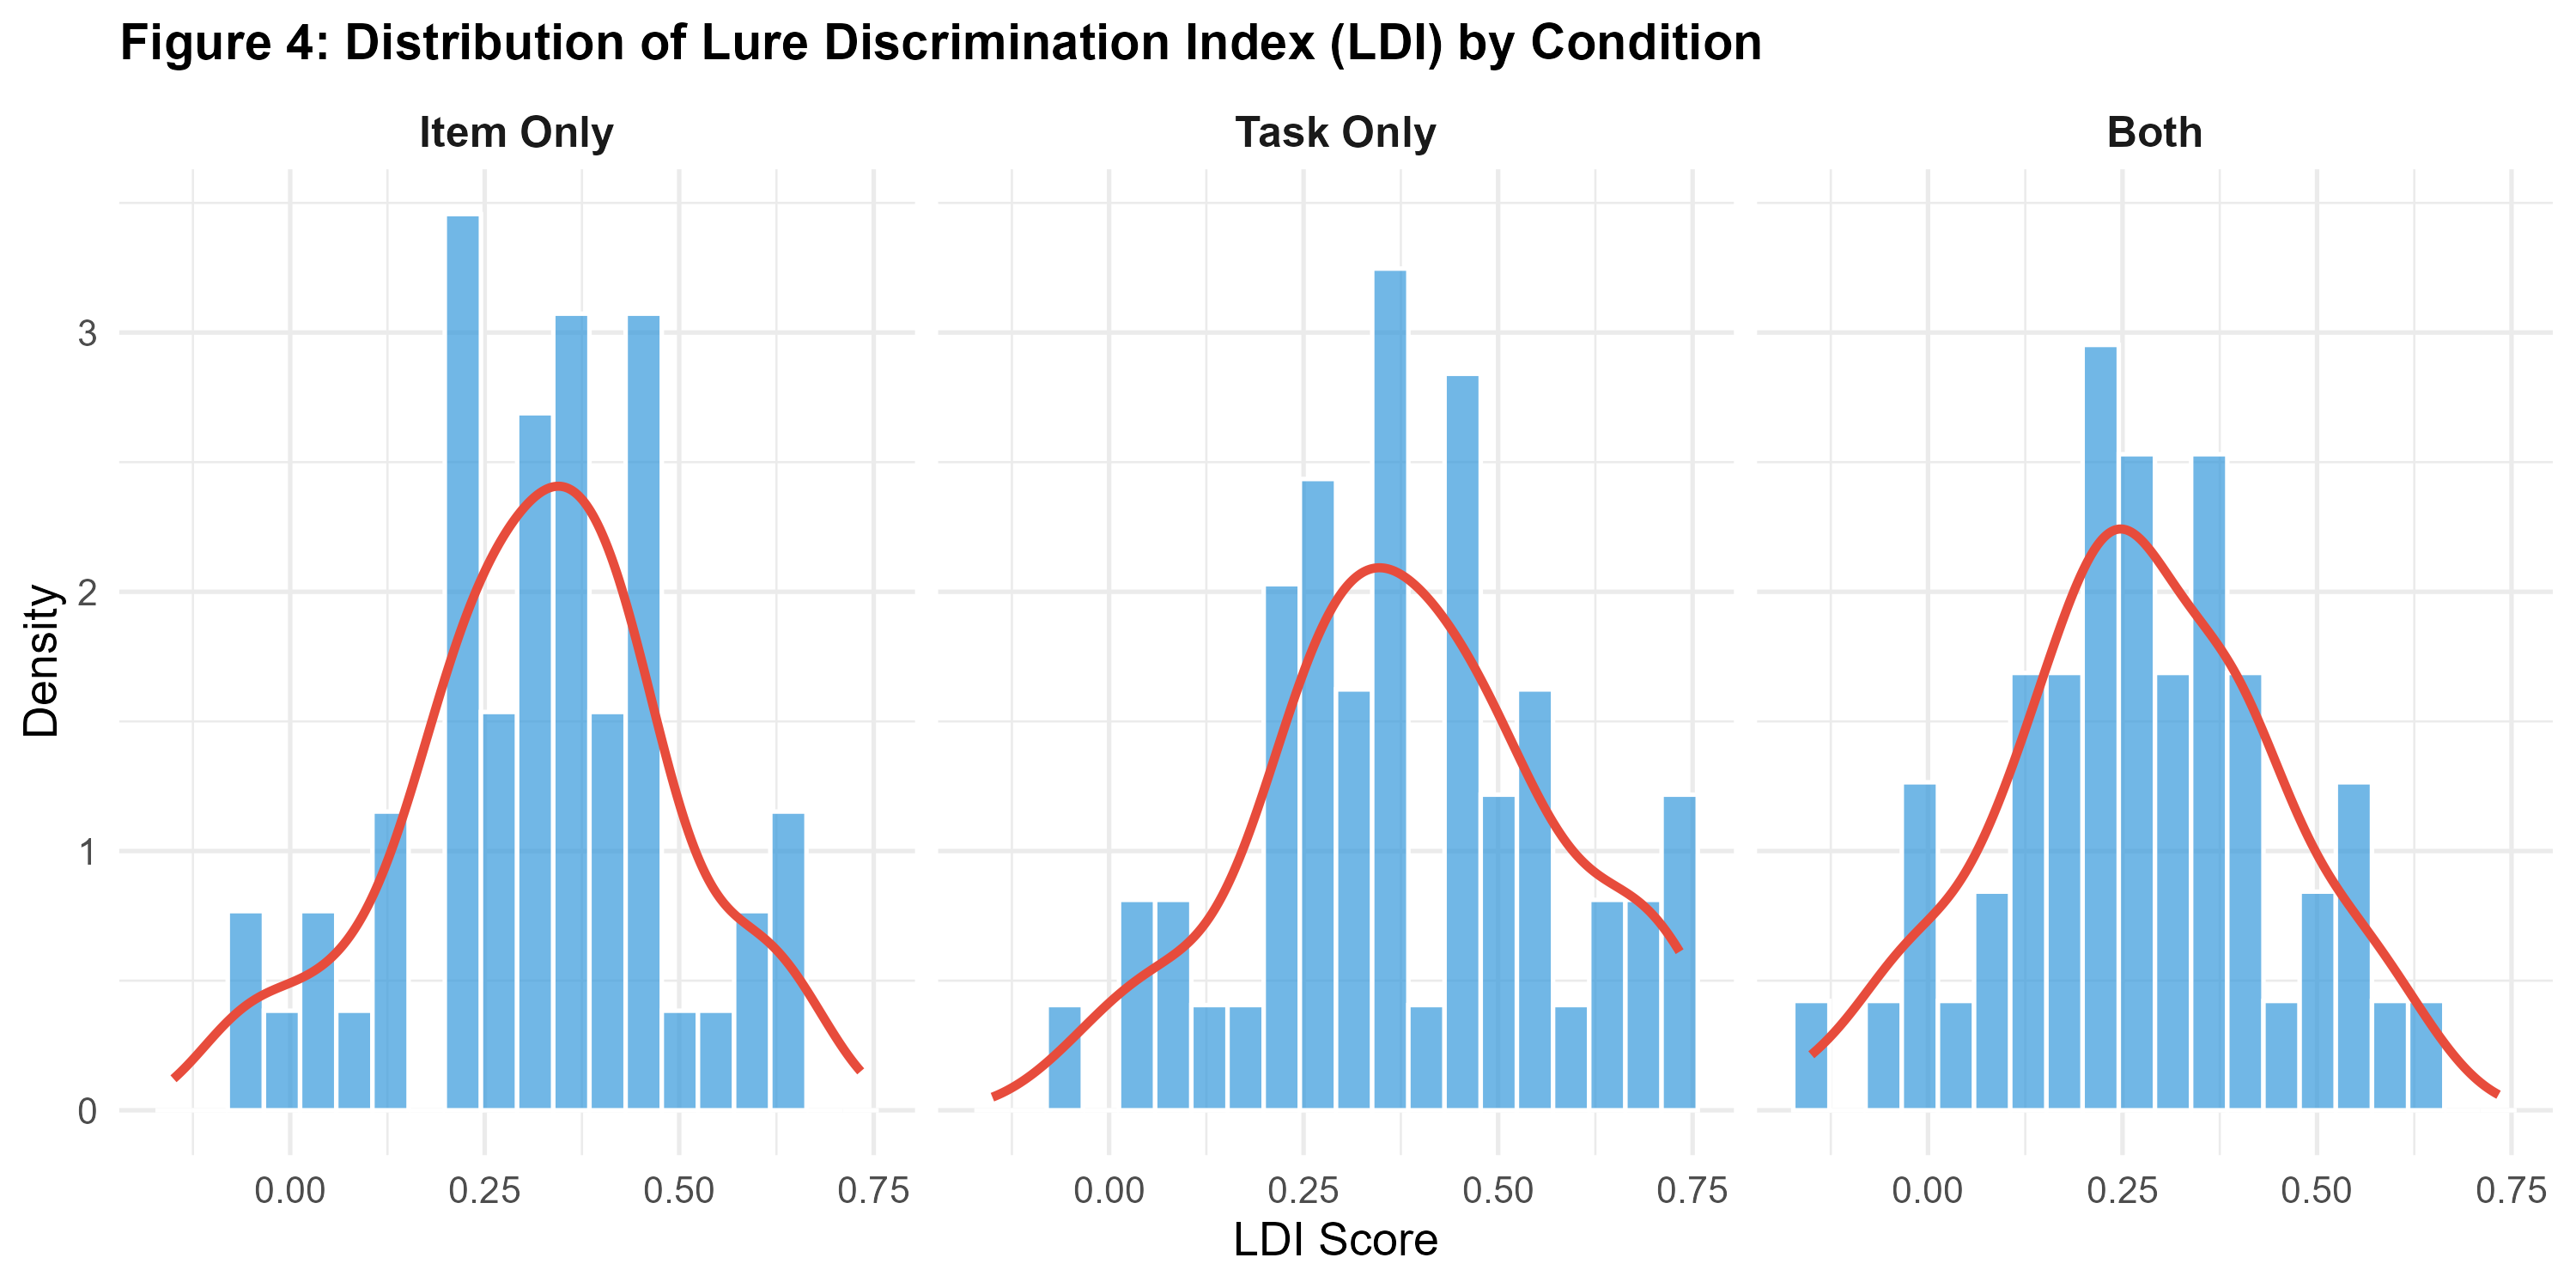
\includegraphics[width=\textwidth]{figures/fig4_ldi_distribution.png}
        \caption{LDI histograms with density overlay}
    \end{subfigure}
    \hfill
    \begin{subfigure}[t]{0.48\textwidth}
        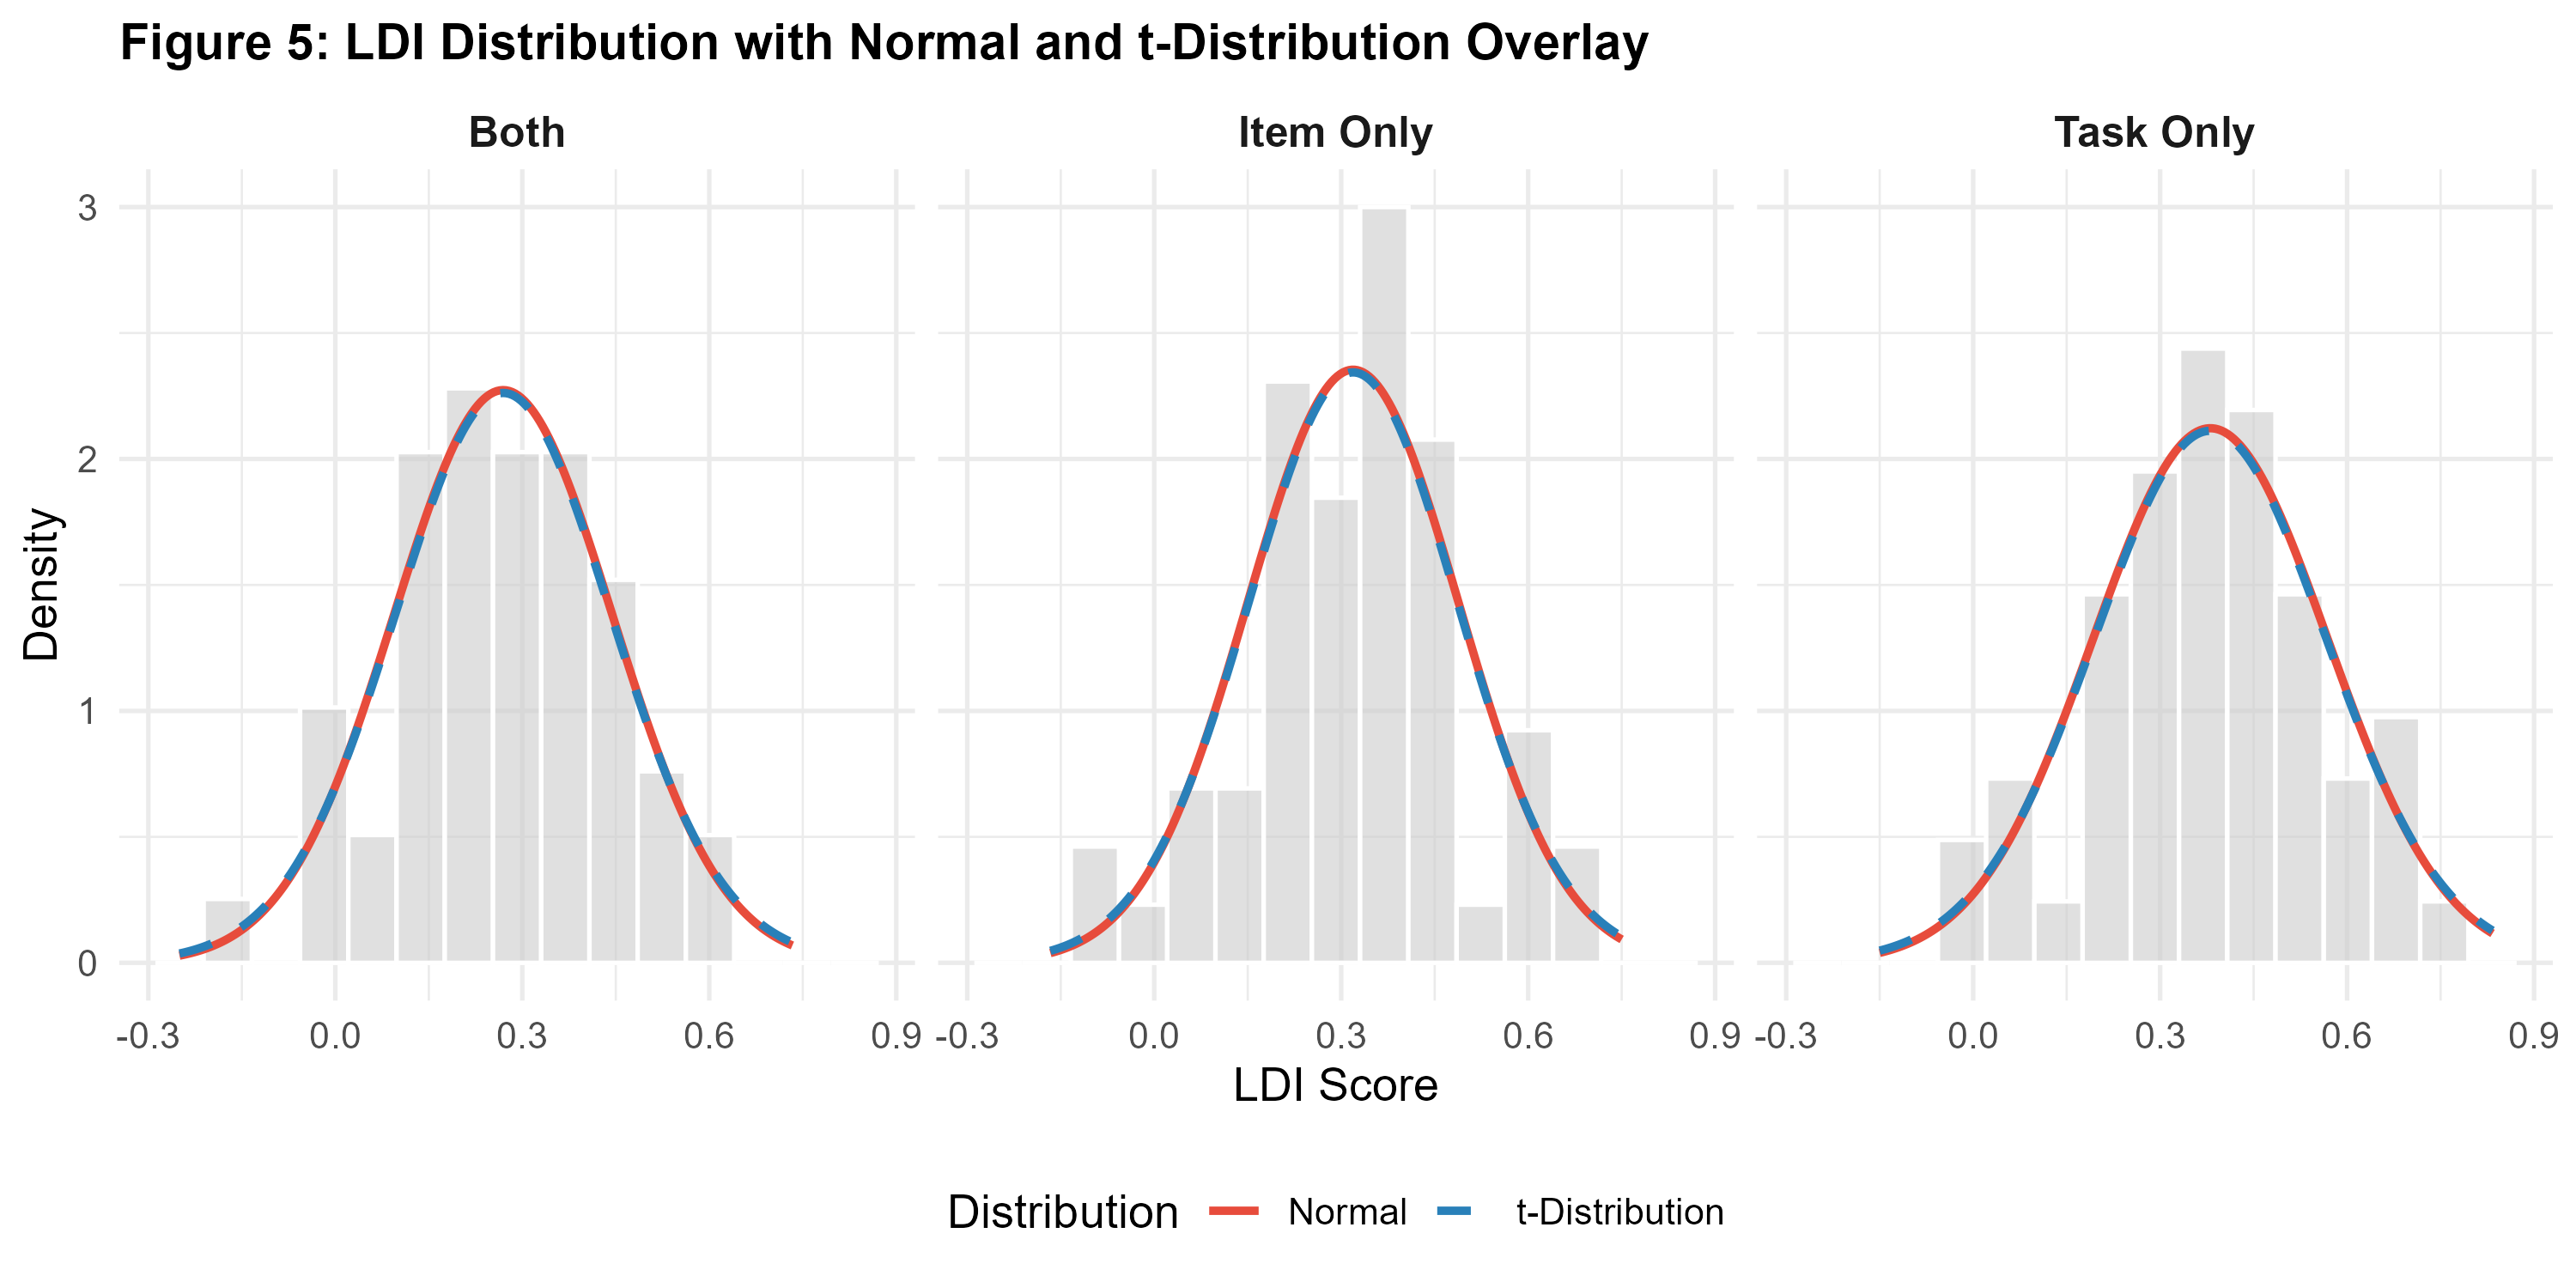
\includegraphics[width=\textwidth]{figures/fig5_normal_t_comparison.png}
        \caption{Normal vs.\ $t$-distribution fit}
    \end{subfigure}
    \caption{Distribution analysis of LDI scores by condition.}
    \label{fig:distributions}
\end{figure}

\subsection{Reaction Time Analysis}

Table~\ref{tab:rt} summarizes RTs by stimulus type. Lures elicited the longest RTs across conditions (2.338--2.831~s), consistent with greater decision difficulty. Median RTs were substantially lower than means (e.g., Item Only lures: $M = 2.83$~s, $Md = 1.89$~s), reflecting positively skewed RT distributions typical of reaction time data. \textbf{The increased latency specifically for lure items cognitively reflects the elevated computational load and decision conflict required by the hippocampus to override a strong, false feeling of familiarity and correctly orthogonalize the overlapping stimuli.}

\begin{table}[H]
\centering
\caption{Reaction Time (seconds) by Condition and Stimulus Type}
\label{tab:rt}
\footnotesize
\begin{tabular}{llccc}
\toprule
\textbf{Condition} & \textbf{Stimulus} & \textbf{Mean} & \textbf{SD} & \textbf{Median} \\
\midrule
\multirow{3}{*}{Item Only} & Target & 2.520 & 2.714 & 1.698 \\
                           & Lure   & 2.831 & 3.040 & 1.889 \\
                           & Foil   & 2.643 & 3.190 & 1.836 \\
\midrule
\multirow{3}{*}{Task Only} & Target & 2.096 & 2.133 & 1.499 \\
                           & Lure   & 2.338 & 1.901 & 1.708 \\
                           & Foil   & 2.278 & 1.822 & 1.691 \\
\midrule
\multirow{3}{*}{Both}      & Target & 2.192 & 2.142 & 1.578 \\
                           & Lure   & 2.388 & 2.264 & 1.765 \\
                           & Foil   & 2.426 & 2.320 & 1.708 \\
\bottomrule
\end{tabular}
\end{table}

\begin{figure}[H]
    \centering
    \begin{subfigure}[t]{0.48\textwidth}
        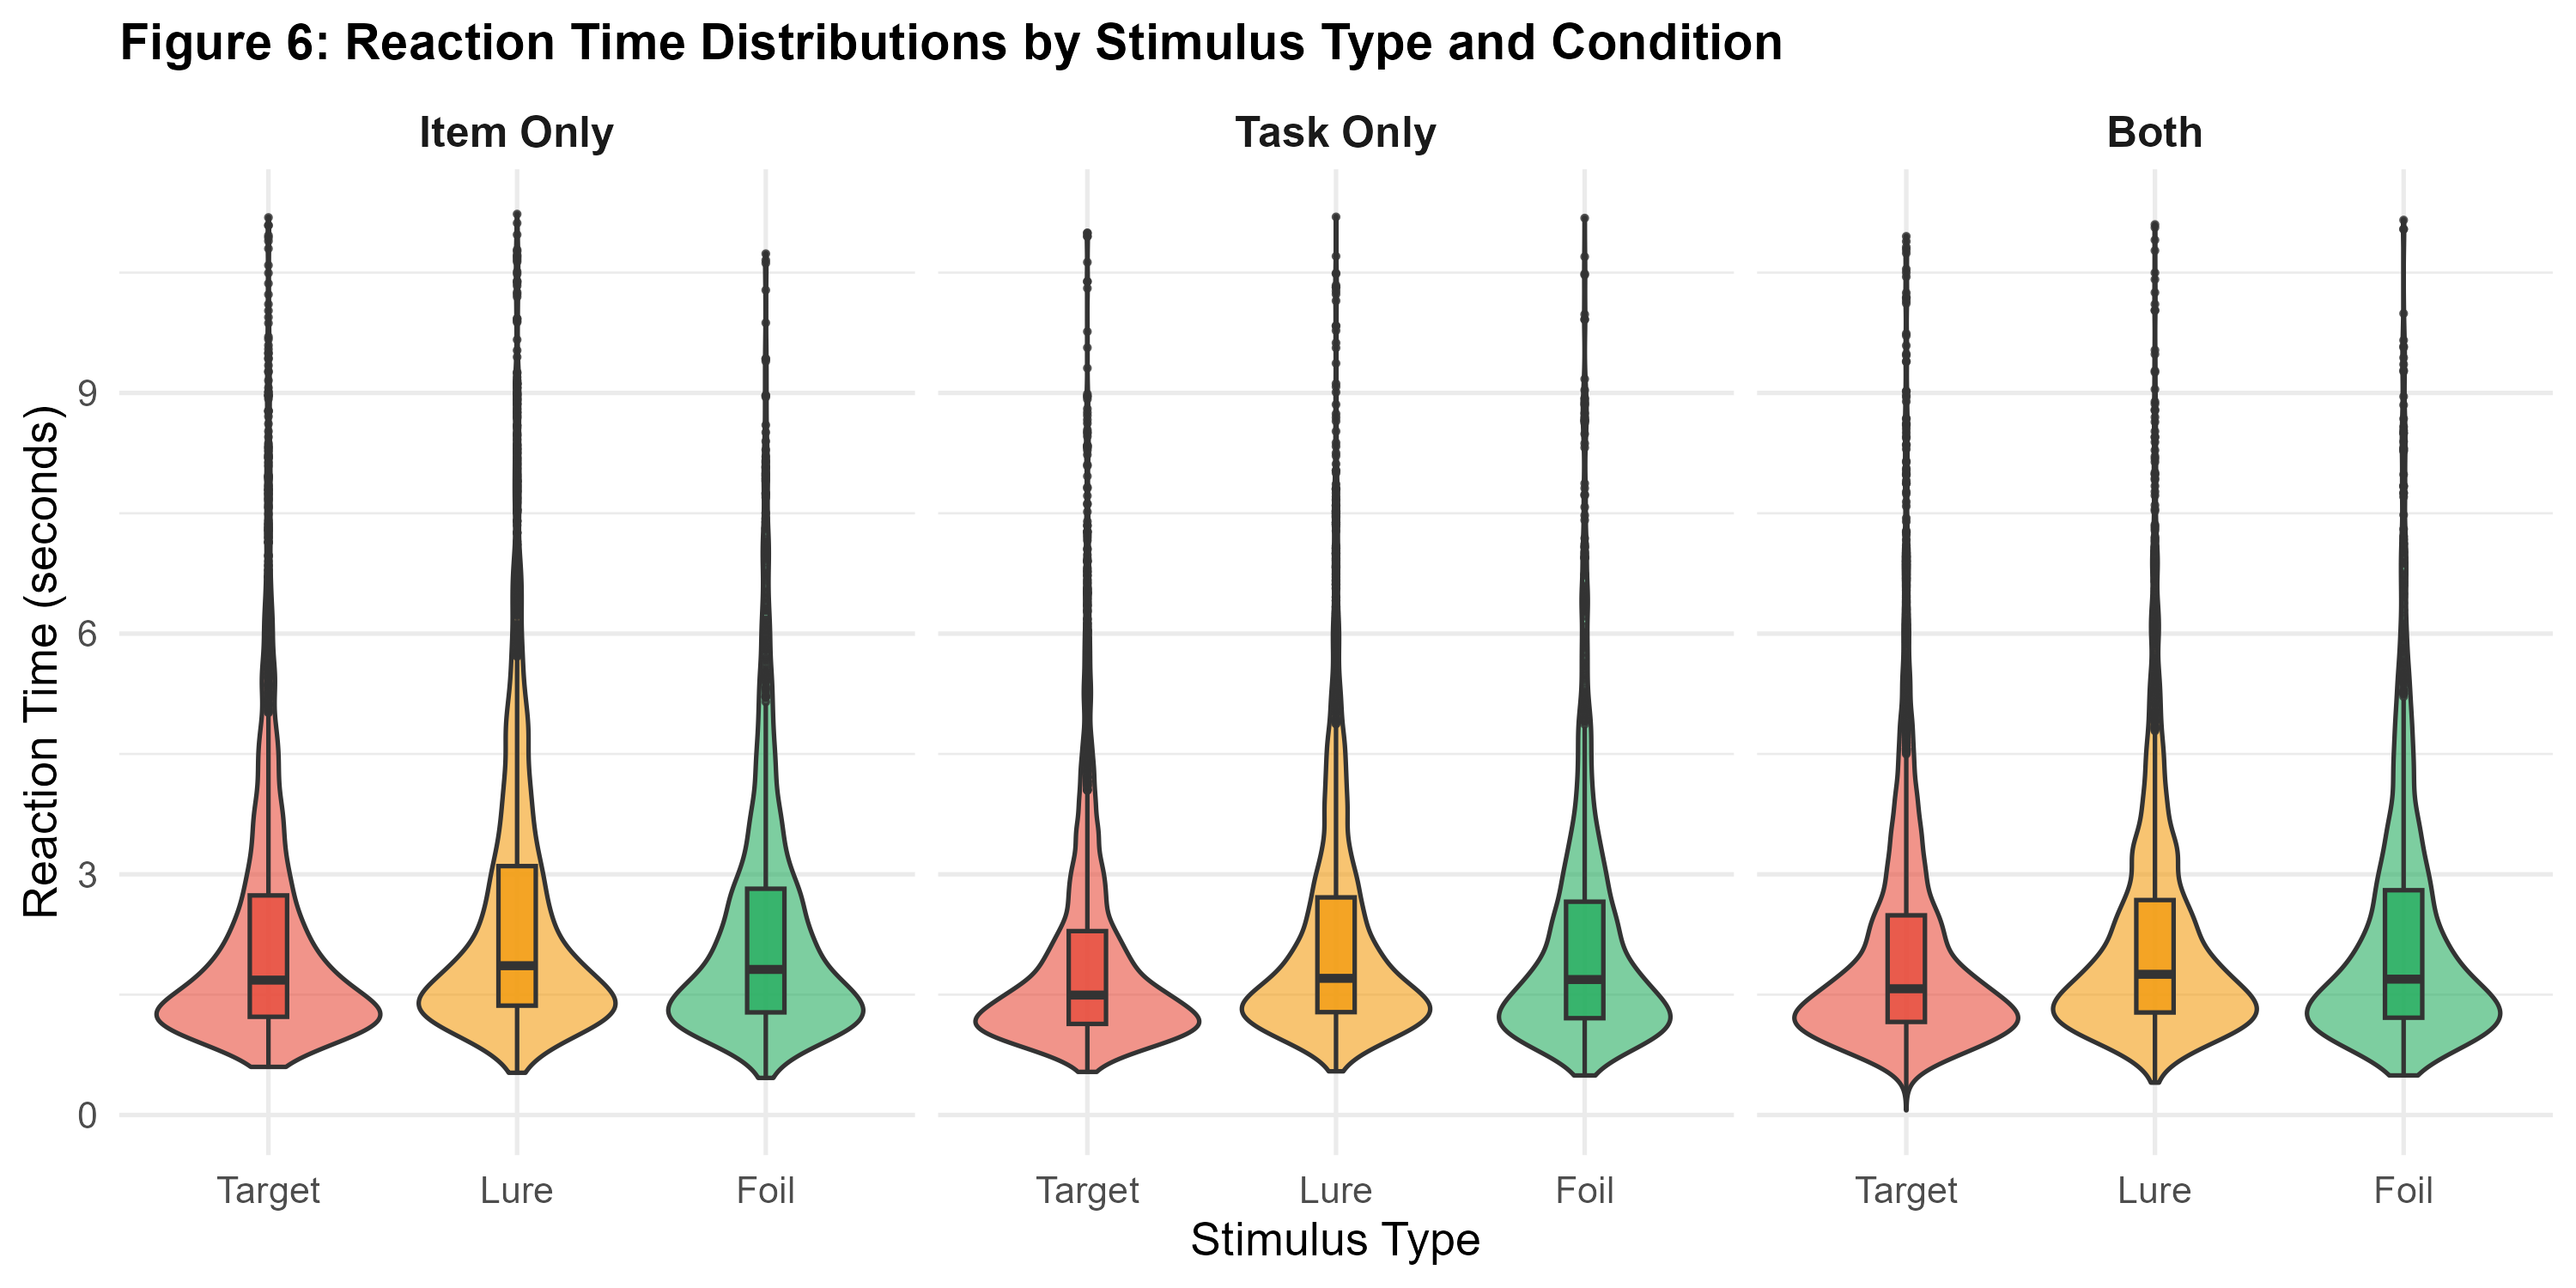
\includegraphics[width=\textwidth]{figures/fig6_rt_violin.png}
        \caption{RT by stimulus type}
    \end{subfigure}
    \hfill
    \begin{subfigure}[t]{0.48\textwidth}
        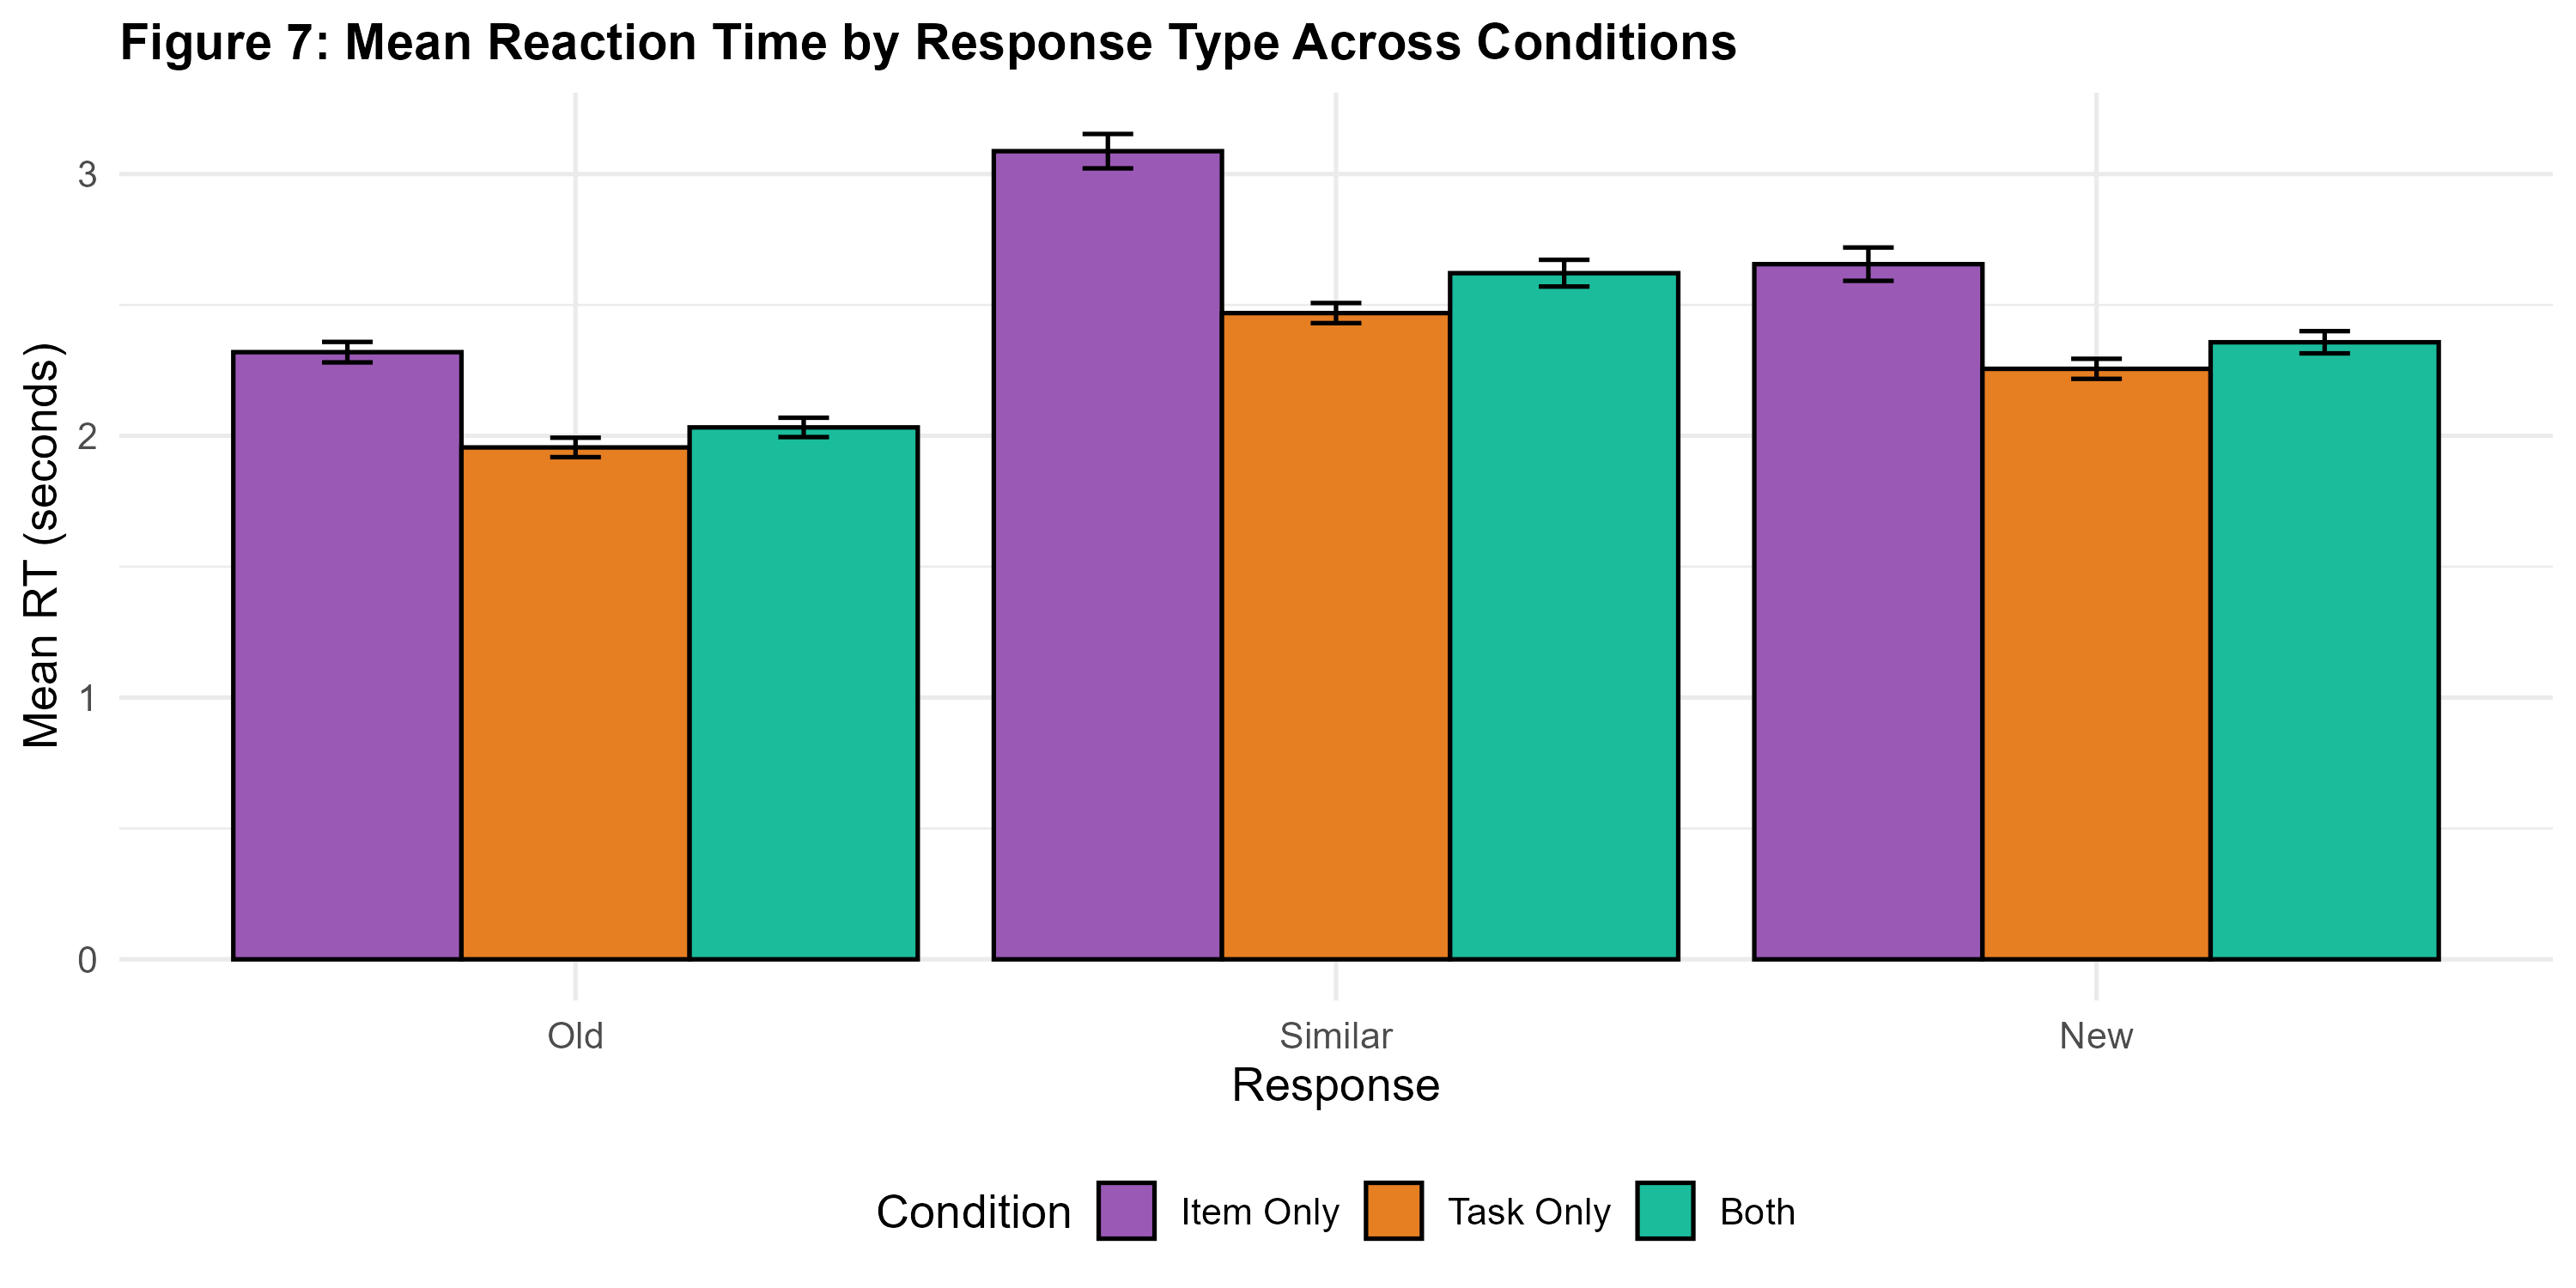
\includegraphics[width=\textwidth]{figures/fig7_rt_by_response.png}
        \caption{Mean RT ($\pm$ SE) by response type}
    \end{subfigure}
    \caption{Reaction time distributions across conditions.}
    \label{fig:rt_figs}
\end{figure}

\subsection{Similarity Bin Analysis}
\label{sec:bins}

Figure~\ref{fig:bins_scatter} (left) shows response proportions as a function of lure similarity. Consistent with \textbf{Hypothesis~3} and the pattern separation framework, more similar lures (Bin~1) were more often falsely endorsed as ``Old,'' while less similar lures (Bin~5) were more readily identified as ``Similar'' or ``New.'' This graded pattern was consistent across all conditions, providing strong support for $H_1$. \textbf{This parametric response shift validates the core mechanism of the MST paradigm, clearly demonstrating that as sensory and conceptual overlap increases, the neural network's ability to maintain distinct representations is increasingly taxed, resulting in higher interference.}

\begin{figure}[H]
    \centering
    \begin{subfigure}[t]{0.48\textwidth}
        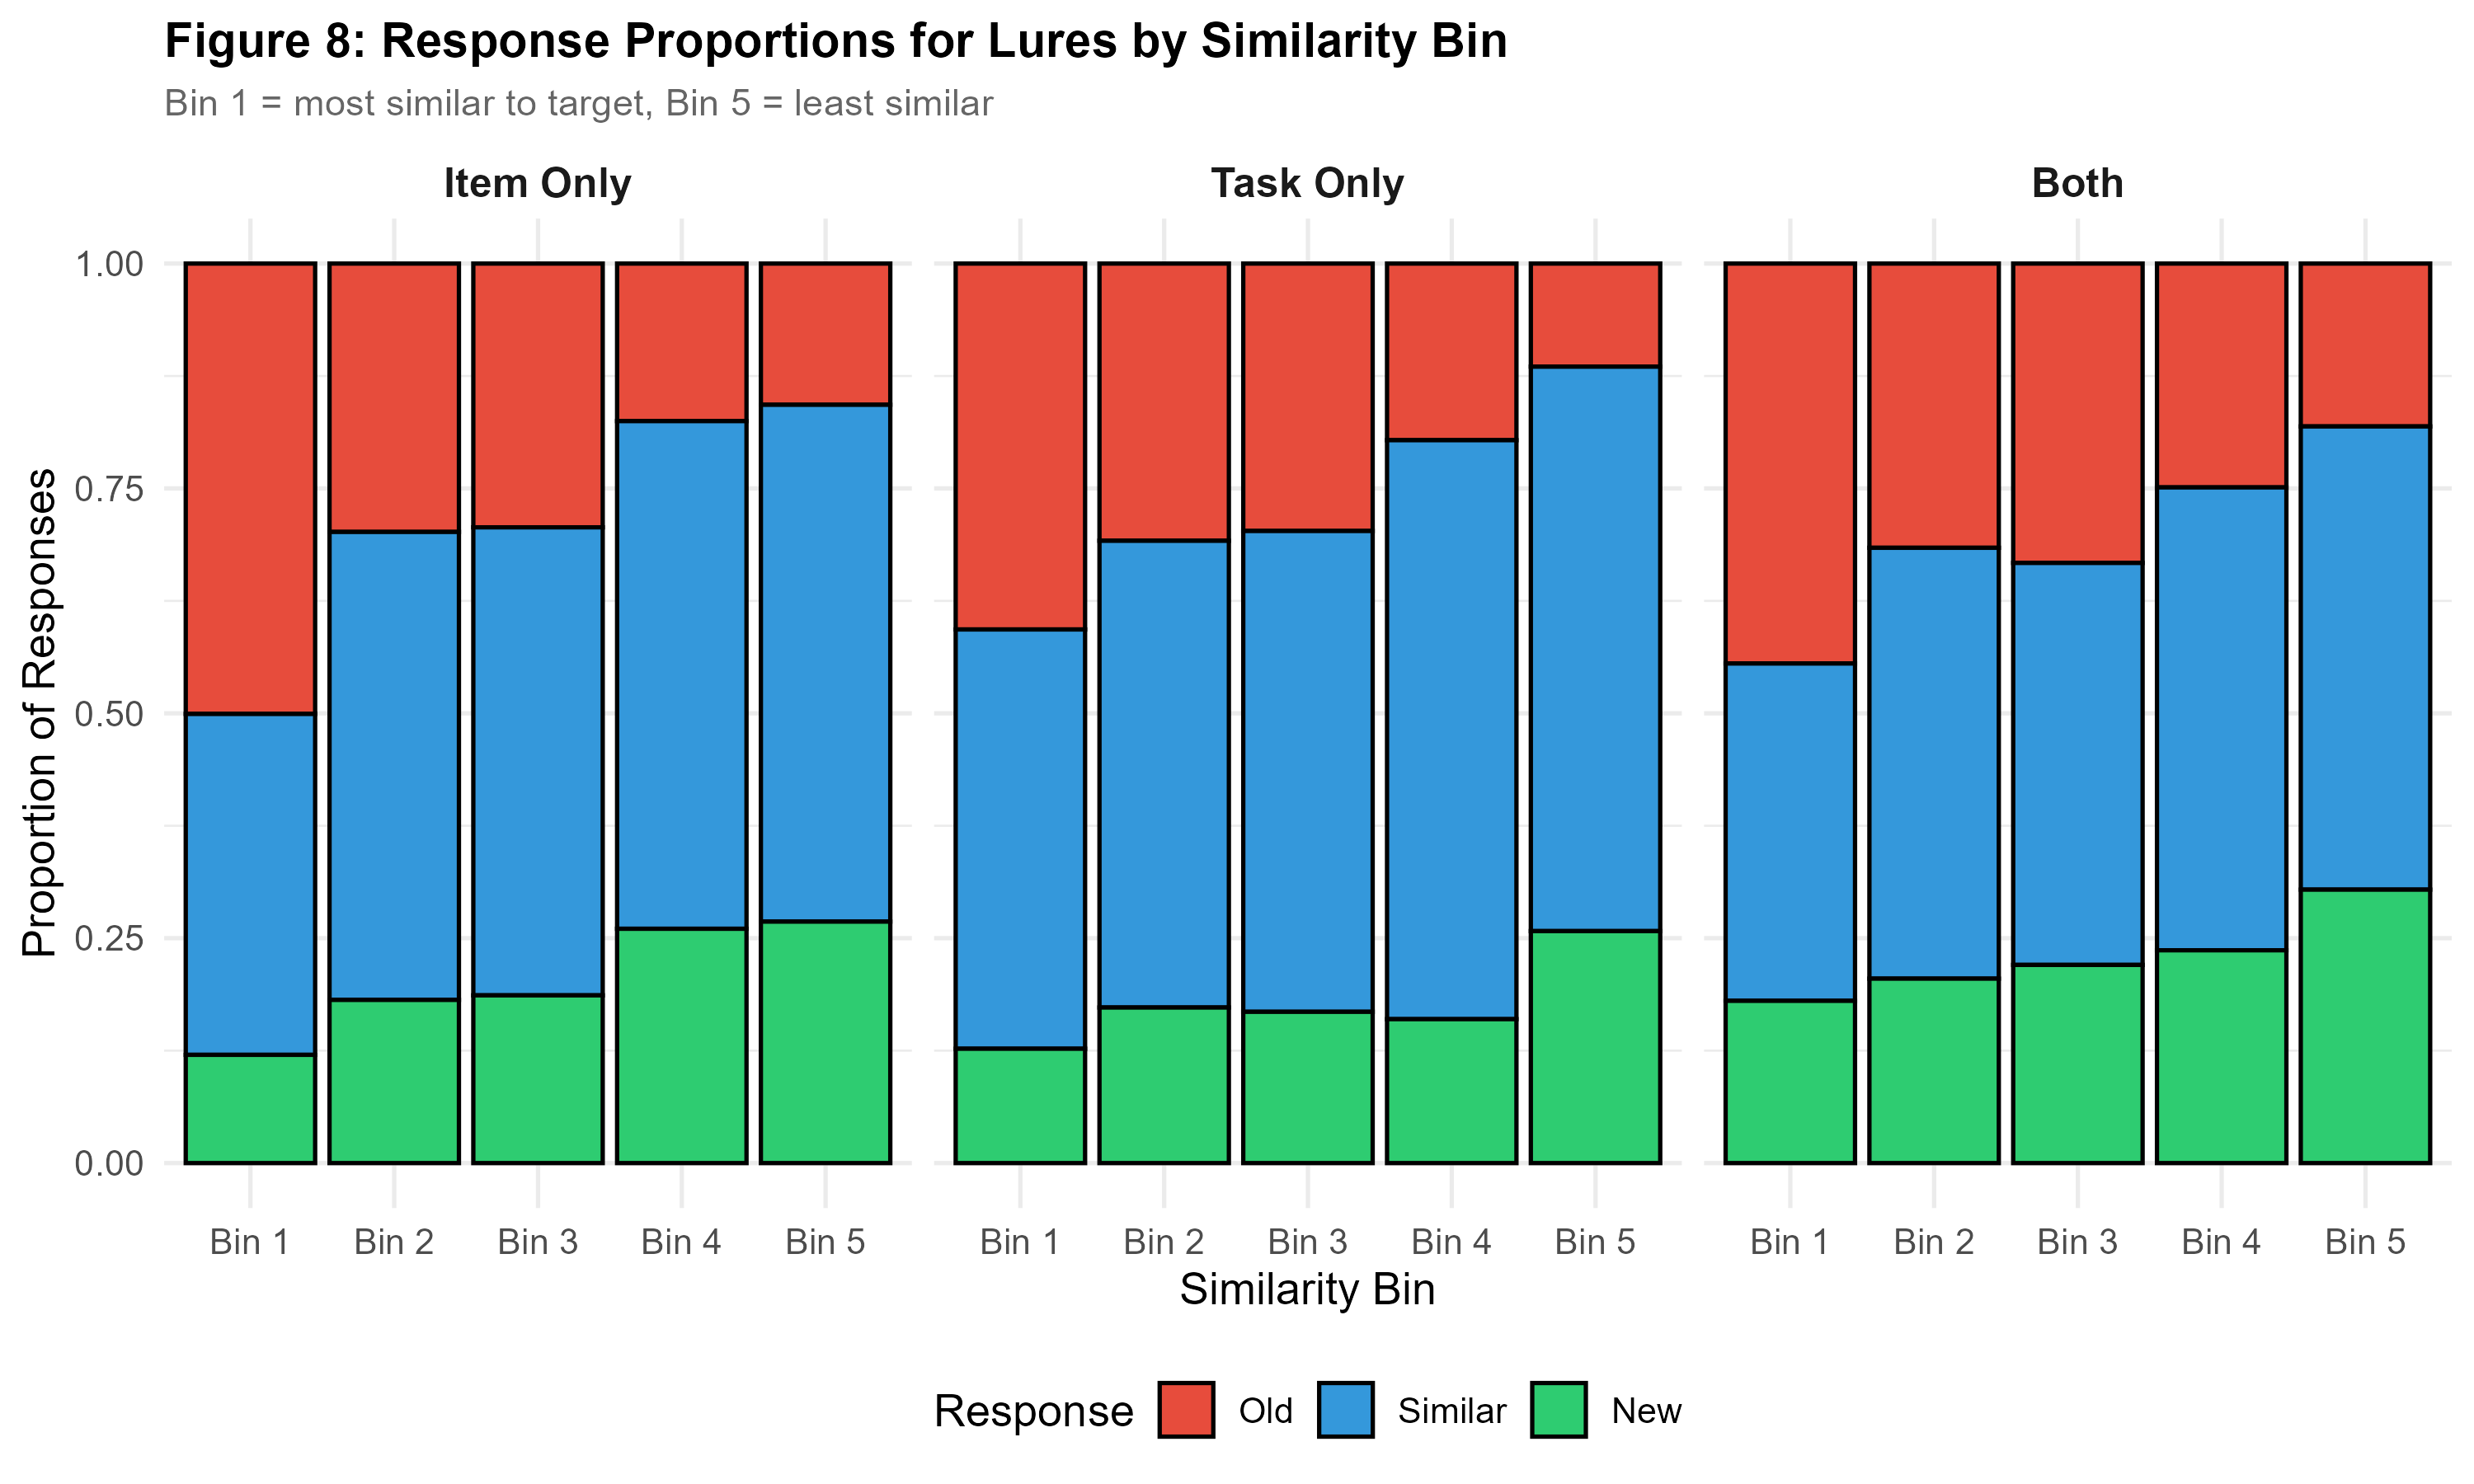
\includegraphics[width=\textwidth]{figures/fig8_bin_performance.png}
        \caption{Lure responses by similarity bin}
    \end{subfigure}
    \hfill
    \begin{subfigure}[t]{0.48\textwidth}
        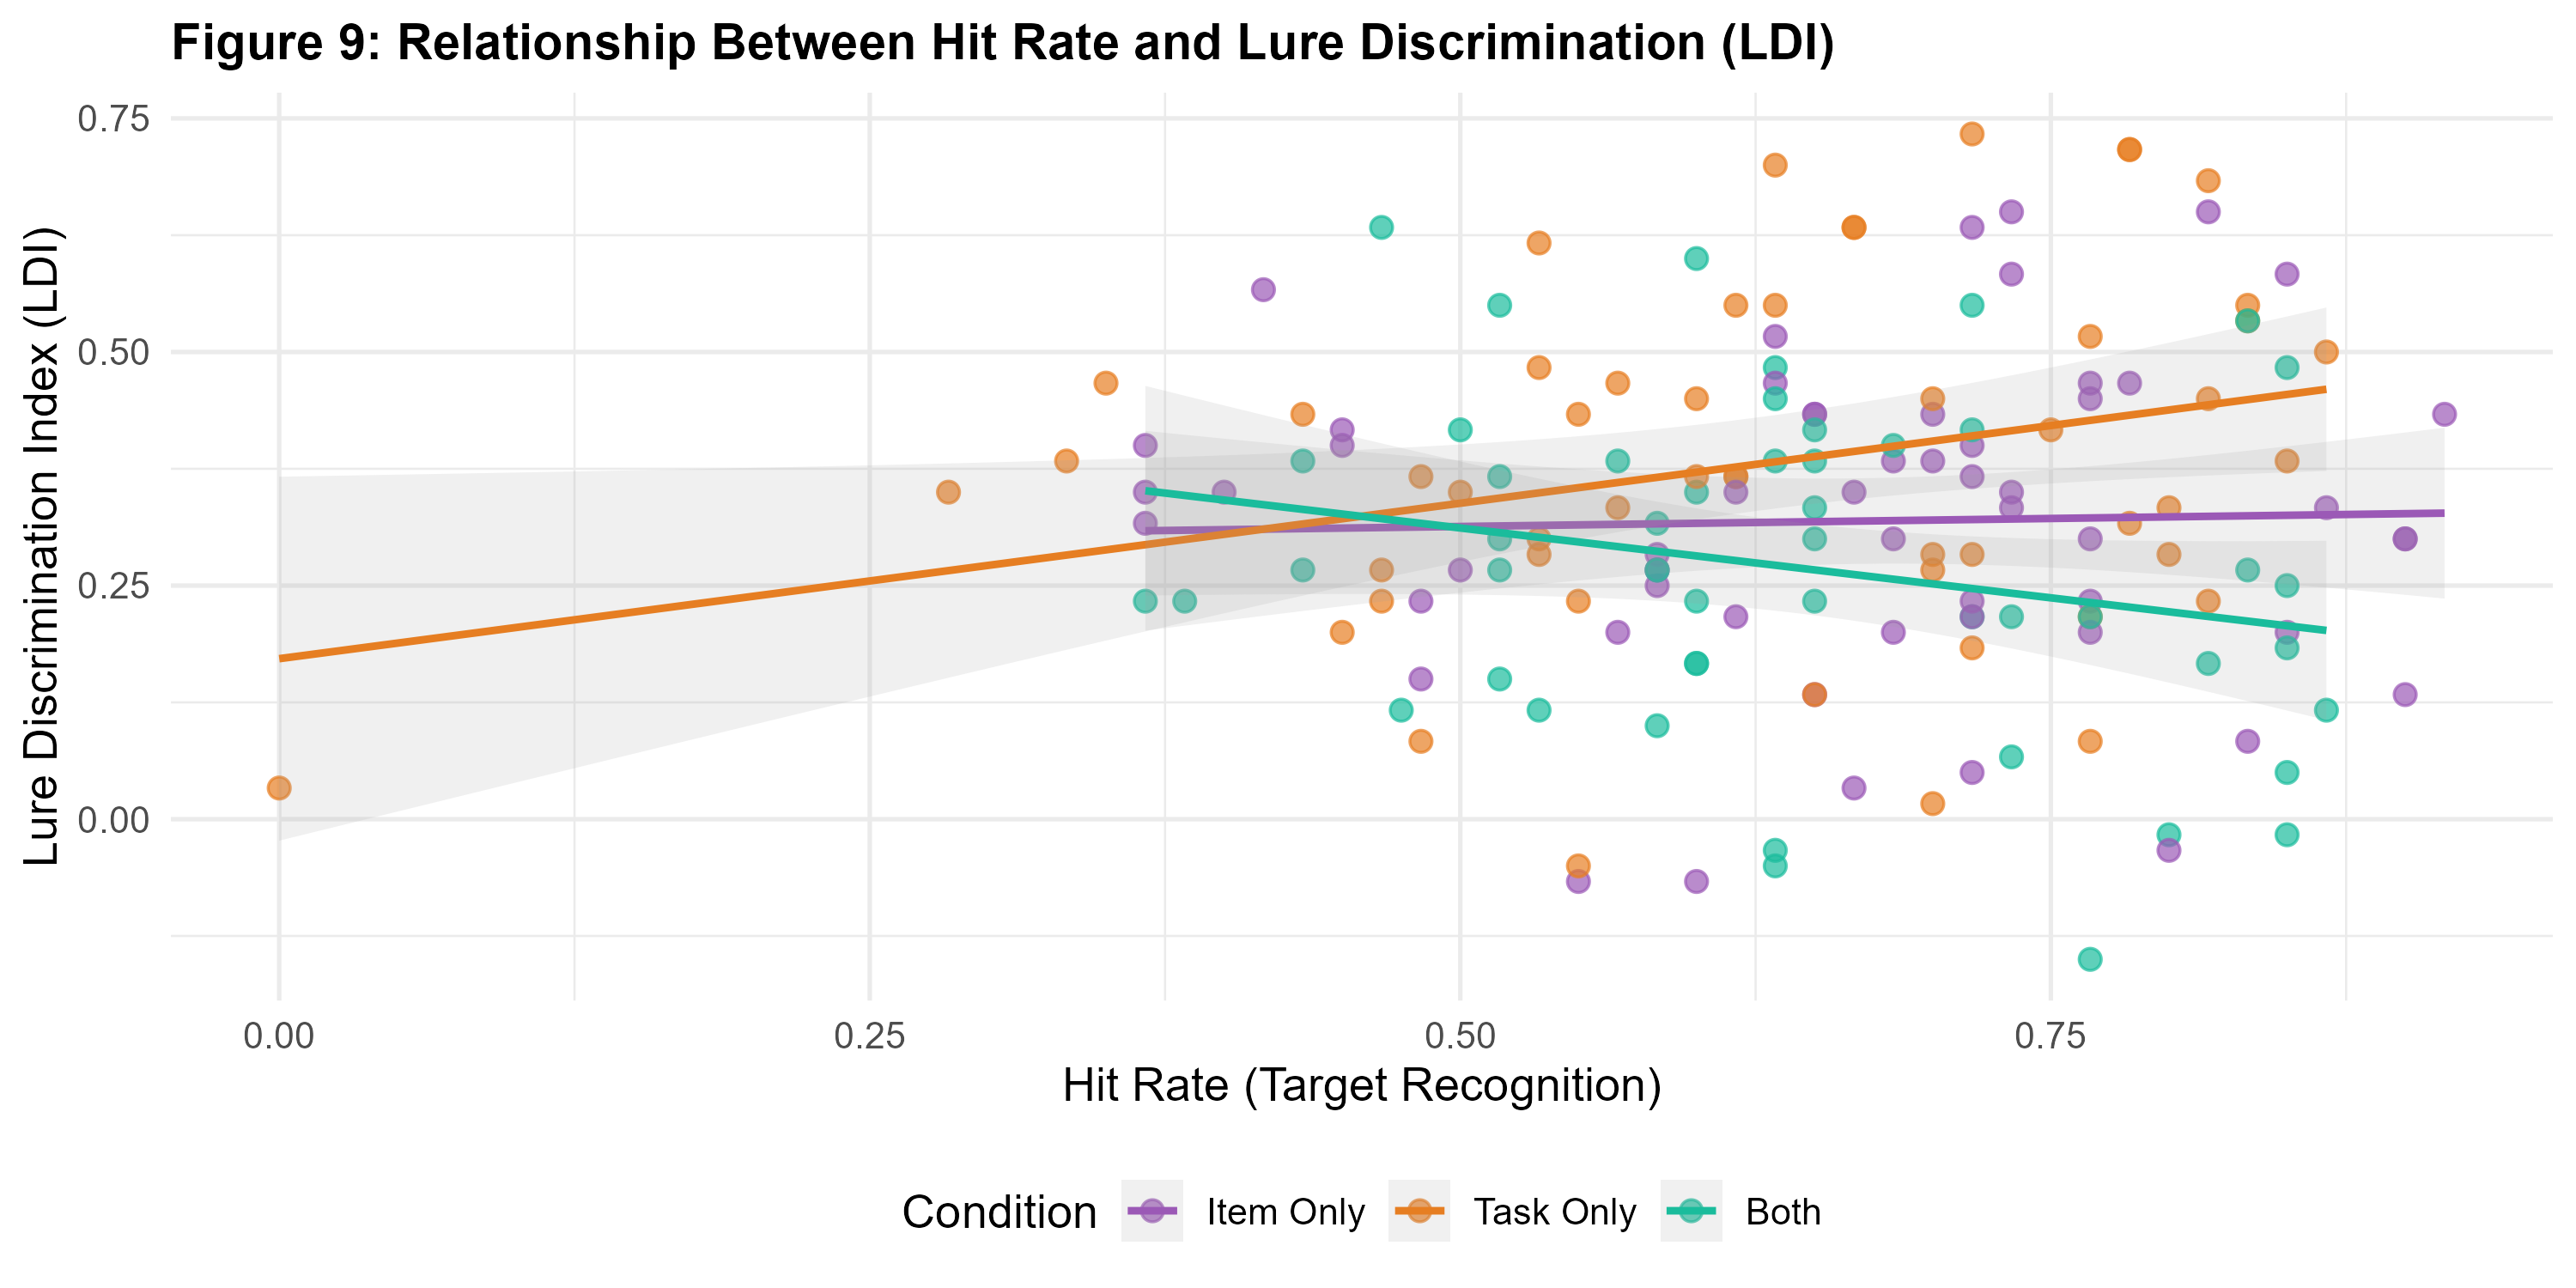
\includegraphics[width=\textwidth]{figures/fig9_hit_vs_ldi.png}
        \caption{Hit Rate vs.\ LDI relationship}
    \end{subfigure}
    \caption{Similarity bin analysis and Hit Rate--LDI relationship by condition.}
    \label{fig:bins_scatter}
\end{figure}

\subsection{Lure Position Analysis}

Lure items appeared at different temporal positions (pre, mid, post) relative to target presentations. Table~\ref{tab:pos_perf} arrays response proportions across these positions. Discrimination performance (proportion of ``Similar'' responses) remained remarkably stable across temporal positions within each condition. \textbf{This cognitive stability indicates that within the constraints of this specific task setup, pattern separation capacity is highly robust; it does not suffer significantly from either short-term memory decay over the testing block or proactive interference caused by encountering numerous intervening stimuli.} Task Only participants maintained the highest ``Similar'' response rate across all positions (.562--.581).

\begin{figure}[H]
    \begin{minipage}[c]{0.5\textwidth}
        \centering
        \captionof{table}{Lure Response Proportions by Temporal Position}
        \label{tab:pos_perf}
        \footnotesize
        \begin{tabular}{llccc}
        \toprule
        \textbf{Condition} & \textbf{Pos.} & \textbf{Old} & \textbf{Similar} & \textbf{New} \\
        \midrule
        \multirow{3}{*}{Item} & pre  & .299 & .504 & .197 \\
                              & mid  & .286 & .520 & .195 \\
                              & post & .284 & .504 & .212 \\
        \midrule
        \multirow{3}{*}{Task} & pre  & .250 & .581 & .169 \\
                              & mid  & .258 & .562 & .180 \\
                              & post & .235 & .579 & .186 \\
        \midrule
        \multirow{3}{*}{Both} & pre  & .326 & .464 & .210 \\
                              & mid  & .289 & .483 & .228 \\
                              & post & .301 & .450 & .249 \\
        \bottomrule
        \end{tabular}
    \end{minipage}
    \hfill
    \begin{minipage}[c]{0.48\textwidth}
        \centering
        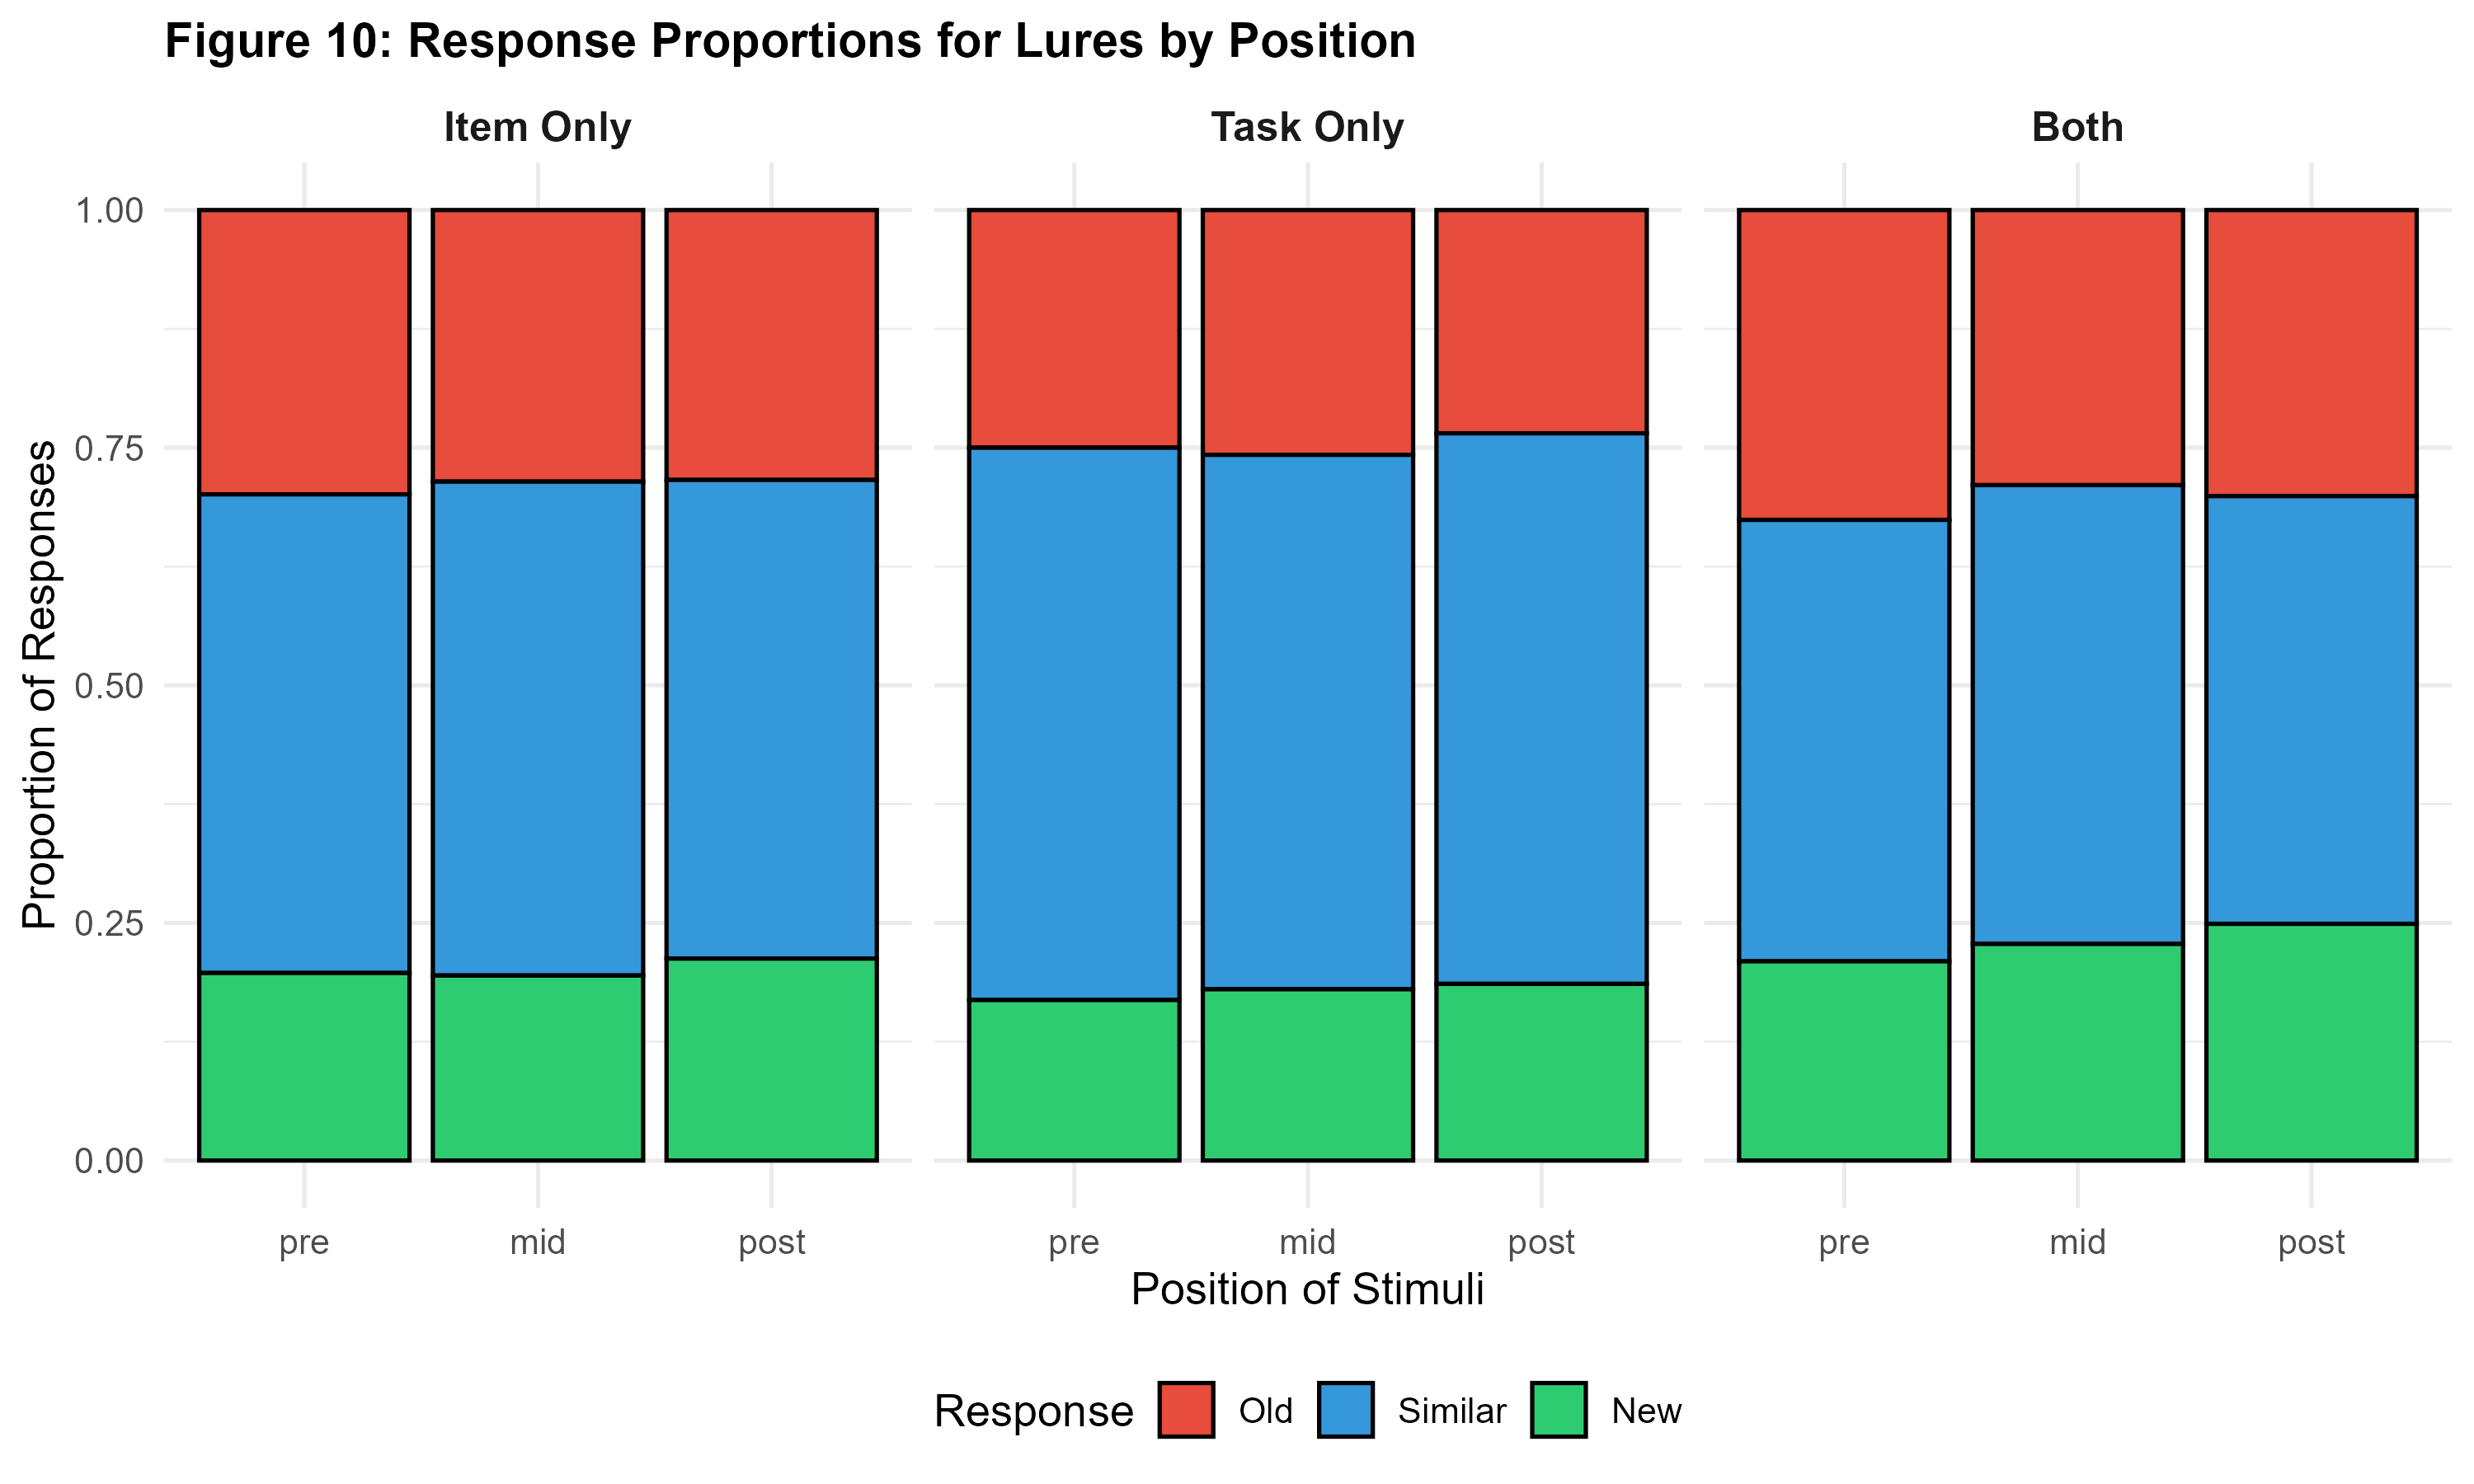
\includegraphics[width=\textwidth]{figures/fig10_pos_performance.png}
        \caption{Lure responses by position.}
        \label{fig:pos_performance}
    \end{minipage}
\end{figure}

\subsection{Overall Accuracy}

Task Only showed the highest overall accuracy (.636), driven by the highest lure identification rate (.574). Both showed the lowest overall accuracy (.592) with the lowest lure identification (.466). Item Only had the highest target accuracy (.669) but moderate lure accuracy (.509).

% ============================================================
% CONCLUSION
% ============================================================
\section{Conclusion}

This analysis of 160 MST participants across three encoding conditions reveals: 
\begin{enumerate}
    \item \textbf{reliable pattern separation}---LDI was significantly above zero in all conditions (all $p < .001$, $d > 1.5$)
    \item \textbf{strong recognition memory}---REC ranged from .594 to .634 (all $t > 24$, $p < .001$)
    \item \textbf{similarity-graded lure discrimination}---bin analysis revealed the expected graded effect of target-lure similarity
    \item \textbf{stable position effects}---lure discrimination was consistent across pre, mid, and post presentation positions
    \item \textbf{positively skewed RTs}---lures elicited longer RTs than targets, reflecting greater decision uncertainty.
\end{enumerate}
\textbf{Limitations:} This report is limited to descriptive statistics; no participant-level outlier exclusion was applied. 

\textbf{Future directions} (Report~2): Formal between-group ANOVA comparisons, condition $\times$ bin mixed-effects models, signal detection analyses ($d'$, criterion $c$), and correlation analyses of encoding--recognition relationships.

% ============================================================
% TEAM CONTRIBUTIONS
% ============================================================
\section{Team Contributions}

The analysis and report were collaborative efforts across all three team members. The specific contributions are outlined below.

\textbf{Sourav Nath} was responsible for data loading and preprocessing, writing R code to programmatically ingest per-participant CSV files, classify stimuli (Targets, Lures, Foils) via suffix-based matching, and map lures to similarity bins. He also computed the Hit Rate, False Alarm Rate, and Correct Rejection Rate at the per-participant level, and contributed to the write-up of the Methods and Overall Performance sections.

\textbf{Piyush Kumar Agarwal} implemented the computation of the Lure Discrimination Index (LDI) and Recognition Memory (REC) metrics, and ran the one-sample $t$-tests with Cohen's $d$ effect sizes for Hypotheses~1 and~2. He also produced the reaction time analysis (including 99th-percentile outlier trimming) and the RT figures (violin plots and mean RT bar plots), and managed the GitHub repository and version control for the project.

\textbf{Rajarshi Chatterjee} led the visualization of the similarity bin analysis and temporal position analysis, producing the corresponding figures using \texttt{ggplot2}. He further conducted the overall accuracy and lure position analyses, generated the Hit Rate vs.\ LDI scatter plots, and was primarily responsible for writing the Results and Conclusion sections of the report.

\newpage
% ============================================================
% GITHUB REPOSITORY
% ============================================================
\section{GitHub Repository}

All R code, analysis scripts, and data processing pipelines developed for this project are publicly available at the following repository:

\begin{center}
\url{https://github.com/piyukr2/BRSM_project}
\end{center}

% ============================================================
% REFERENCES
% ============================================================
\bibliographystyle{apalike}

\begin{thebibliography}{9}

\bibitem[Bakker et al., 2008]{bakker2008pattern}
Bakker, A., Kirwan, C. B., Miller, M., \& Stark, C. E. L. (2008).
Pattern separation in the human hippocampal CA3 and dentate gyrus.
\textit{Science}, 319(5870), 1640--1642.

\bibitem[Stark et al., 2013]{stark2013mnemonic}
Stark, S. M., Yassa, M. A., Lacy, J. W., \& Stark, C. E. L. (2013).
A task to assess behavioral pattern separation (BPS) in humans: Data from healthy aging and mild cognitive impairment.
\textit{Neuropsychologia}, 51(12), 2442--2449.

\bibitem[Yassa \& Stark, 2011]{yassa2011pattern}
Yassa, M. A., \& Stark, C. E. L. (2011).
Pattern separation in the hippocampus.
\textit{Trends in Neurosciences}, 34(10), 515--525.

\end{thebibliography}

\end{document}